In der geomtrischen Optik wird Licht mit Hilfe des Strahlenmodells des Lichts beschrieben. Dadurch kann man auf rein geomtrische Art Licht mit Linien beschrieben, was für die Beschreibung optischer Abbildungen eine gut geeignete Näherung ist. Somit findet die geometrische Optik in der Beschreibung optischer Systeme, wie Linsen, Fernrohren und Mikroskopen Verwendung. Die vier Axiome der geometrischen Optik folgen unter anderem aus dem fermatischen Prinzip, das die Grundlage der Strahloenoptik darstellt. Es sagt aus, dass Licht in einem Medium zwischen zwei Punkten Wege nimmt, auf denen seine Laufzeit sich bei kleinen Variationen des Weges nicht ändert. \\
Die vier Axiome der geometrischen Optik sind: \\
\begin{itemize}
\item[1.]Axiom: In homogenem Material sind die Lichtstrahlen gerade. \\
\item[2.]Axiom: An der Grenze zwischen zwei homogenen isotropen Materialien wird das Licht im Allgemeinen nach dem Reflexionsgesetz \ref{Reflexionsgesetz} reflektiert und nach dem Brechungsgesetz
\ref{Brechungsgesetz} gebrochen. 
\end{itemize}
    \begin{equation} \label{Reflexionsgesetz}
        \alpha = \beta
    \end{equation}
    
    \begin{equation} \label{Brechungsgesetz}
        n_1 \cdot \sin{\alpha_1} = n_2 \cdot \sin{\alpha_2}
    \end{equation}
    \\
\begin{itemize}
\item[3.]Axiom: Der Strahlengang ist umkehrbar, die Lichtrichtung auf einem Lichtstrahl ist belanglos. \\
\item[4.]Axiom: Die Lichtstrahlen durchkreuzen einander, ohne sich gegenseitig zu beeinflussen. \\
\end{itemize}  
    \begin{figure}
        \centering
        \includegraphics{Geometrische_Optik/Protokoll/fig/Reflexionsgesetz.png}
        \caption{Reflexionsgesetz}
        \label{fig:Reflexionsgesetz}
    \end{figure}
    
    \begin{figure}
        \centering
        \includegraphics{Geometrische_Optik/Protokoll/fig/Brechungsgesetz.png}
        \caption{Brechungsgesetz}
        \label{fig:Brechungsgesetz}
    \end{figure}